%NYU 2019 Grad Computational Physics Homework 6

\documentclass[12pt, graphicx]{article}
\pagestyle{plain}
\baselineskip 18pt
\textwidth 6.5in
\textheight 7.8in
\oddsidemargin 0.1in
\evensidemargin 0.1in
\topmargin 0.3in
\parindent 0pt
\linespread{1.5}
\setlength{\parskip}{2.5mm}

\usepackage{graphicx, psfrag, epsfig}
\usepackage[font = small, format = plain, labelfont = bf, textfont = it, justification = raggedright, singlelinecheck = false]{caption}
\usepackage{subfig}
\usepackage{amsmath, amssymb}
\usepackage{geometry}
%\usepackage[symbol]{footmisc}

\renewcommand\tablename{Table}
\renewcommand\figurename{Fig.}
\renewcommand{\thefootnote}{\fnsymbol{footnote}}


\begin{document}
\title{Computational Physics Homework 6}
\author{Hao Li\footnotemark[2]}
\footnotetext[2]{hl3270@nyu.edu~~UID:N12137527}
\date{\today}


\maketitle

\section*{Problem 1}
The code for Markov chain Monte Carlo simulation of the Ising model on the square lattice for a system of $20\times 20$ spins are available in \textquotedblleft Hw\_6-1.c\textquotedblright. In this code, we first randomly initialize the spin on each site with $\pm 1$. Then we calculate the total magnetization $M$ by 
\begin{equation}
M=\sum_is_i
\end{equation}
and the total energy $E$ by 
\begin{equation}
E=-J\sum_{<ij>}s_is_j
\end{equation}
where $J$ is a positive interaction constant (exchange integral). \par
After initialization, we start to randomly flip a spin each time. For each flip, total energy for the new state $E_j$ is calculated and is compared with that of the previous state $E_i$. The acceptance probability for this step is given from $E_i, E_j$ by 
\begin{equation}
P_a= \begin{cases} 
1 & \mbox{if } E_j\leq E_i, \\
\mathrm{e}^{-\beta(E_j-E_i)} & \mbox{if } E_j>E_i.
\end{cases}
\label{eq:Pa}
\end{equation}
where $\beta=\frac{1}{k_BT}$, $k_B=1$ is the Boltzmann constant, and $T$ is the temperature.\par
This means if $E_j\leq E_i$, this move will always be accepted. However, for $E_j>E_i$, a random number $z\in[0,1)$ is generated uniformly. The move will be accepted if $z<\mathrm{e}^{-\beta(E_j-E_i)}$, while if not, previous state and variables will simply be copied to this step. If the move is accepted, new magnetization will also be calculated and refreshed. \par
In this problem, for each condition, we are going to calculate for $N=10^6$ steps. Exchange integral is set to be $J=1$. We will simulate for temperatures $T=1, 2, 3$, to find the sign of spontaneous magnetization.\par
Starting from low temperature $T=1$, the program was run several times and two optimal and typical results were chosen. Fig. \ref{fig:st1n} and Fig. \ref{fig:st1p} show the development of the spin lattice in this condition, taking samples of step $n=0,10^2,10^4,10^6$, but resulting in nearly entirely negative or positive spins. From these plots we can clearly see that the magnetization is obvious and complete.\par

\begin{figure}[ht]
\centering
\begin{minipage}{0.48\linewidth}
\centering
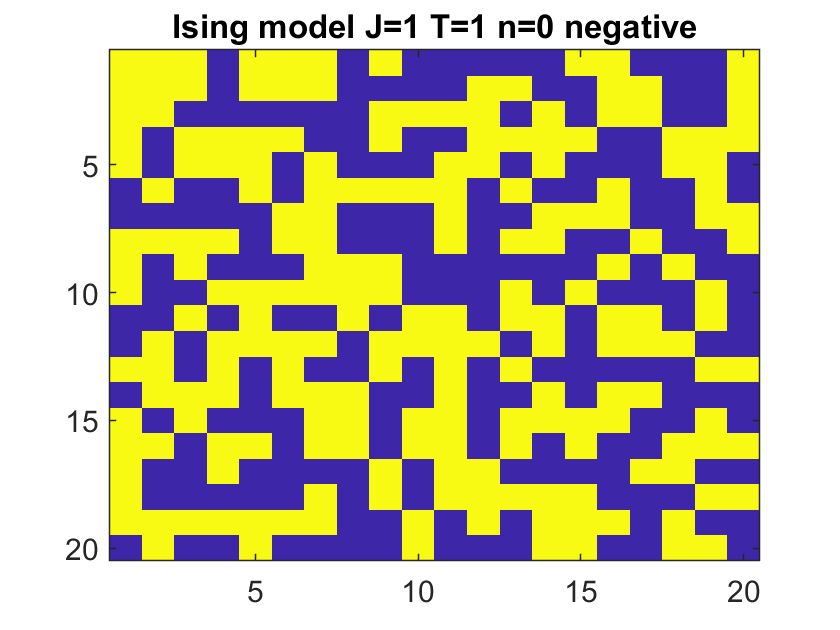
\includegraphics[width = 80mm]{st1n0n.png}
\end{minipage}
\begin{minipage}{0.48\linewidth}
\centering
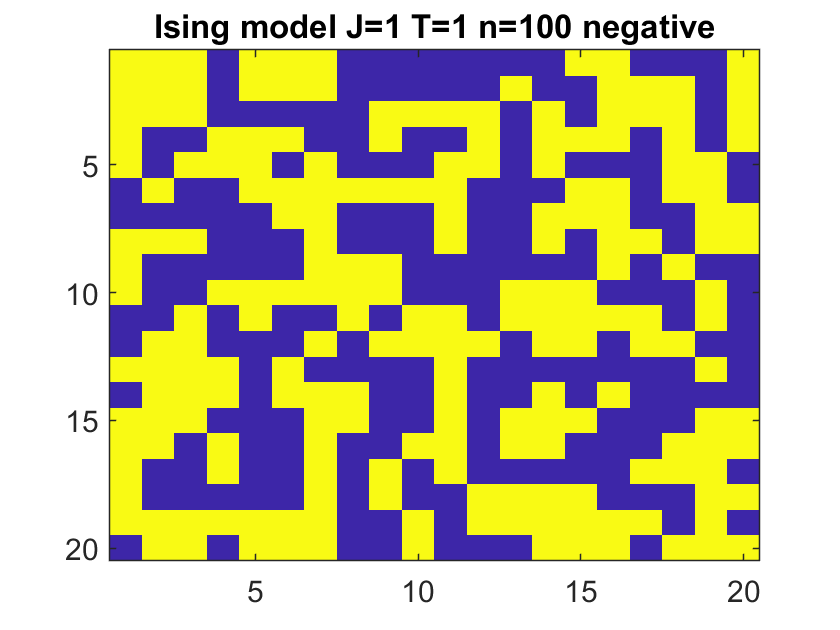
\includegraphics[width = 80mm]{st1n2n.png}
\end{minipage}
\begin{minipage}{0.48\linewidth}
\centering
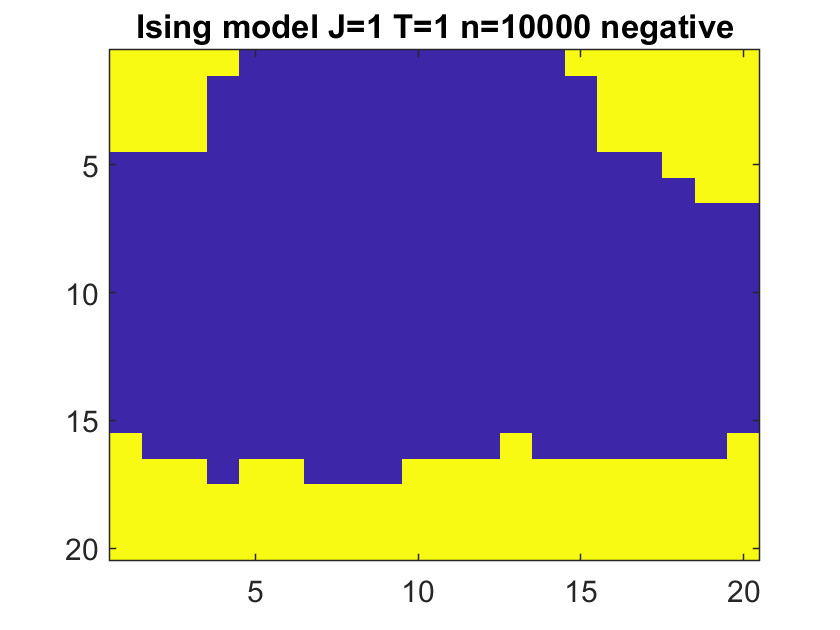
\includegraphics[width = 80mm]{st1n4n.png}
\end{minipage}
\begin{minipage}{0.48\linewidth}
\centering
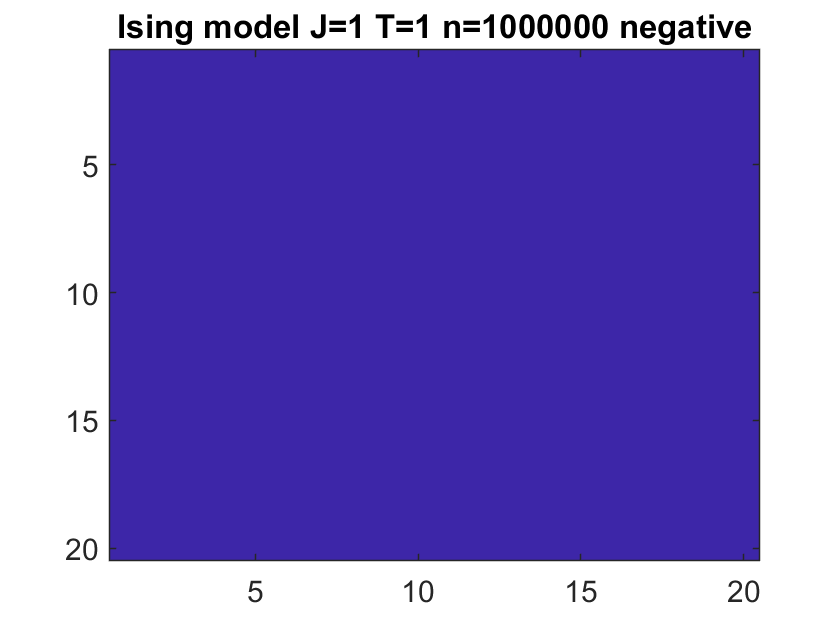
\includegraphics[width = 80mm]{st1n6n.png}
\end{minipage}
\caption{The development of spin latice of the Ising model using Markov chain Monte Carlo simulation. $J=k_B=1$, $T=1$. The program is run for $N=10^6$ steps. Here the states for step $n=0,10^2,10^4,10^6$ are taken as examples. From the plots, it can be implied that at this temperature, spins of the same sign will spontaneously concentrate and at last get nearly completely magnetized to a particular sign. For these plots, the system at last gets completely magnetized to a negative $M$. In this figure, blue correspond to $s_i=1$, and yellow is $s_i=-1$.}
\label{fig:st1n}
\end{figure}

\begin{figure}[ht]
\centering
\begin{minipage}{0.48\linewidth}
\centering
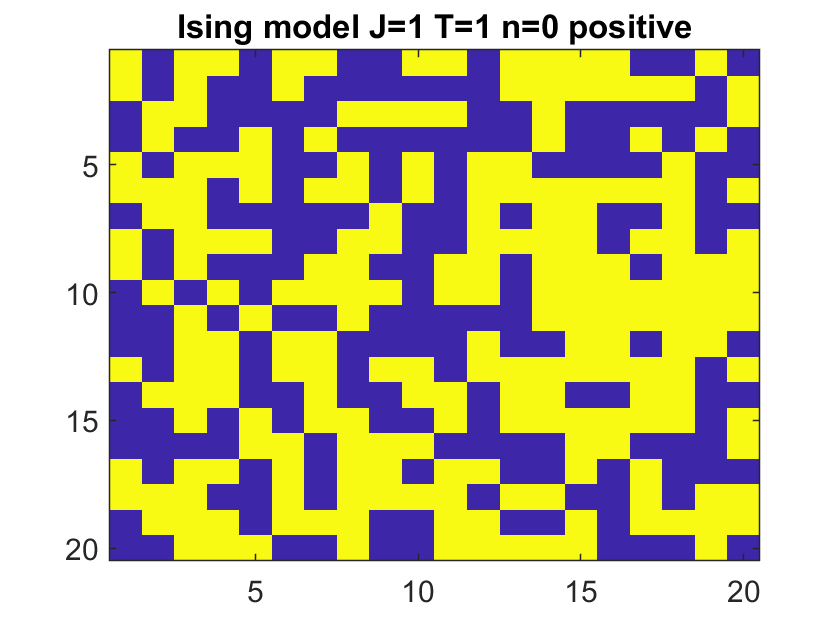
\includegraphics[width = 80mm]{st1n0p.png}
\end{minipage}
\begin{minipage}{0.48\linewidth}
\centering
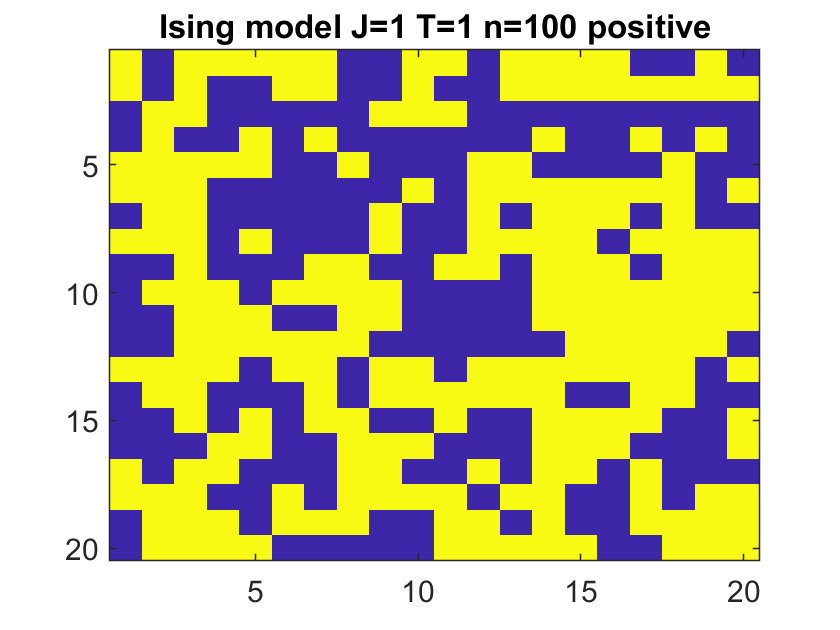
\includegraphics[width = 80mm]{st1n2p.png}
\end{minipage}
\begin{minipage}{0.48\linewidth}
\centering
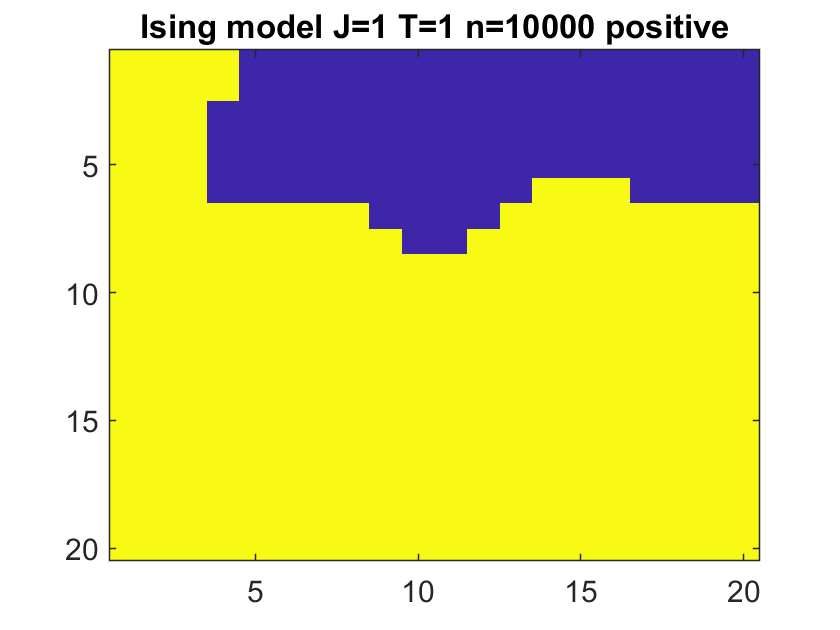
\includegraphics[width = 80mm]{st1n4p.png}
\end{minipage}
\begin{minipage}{0.48\linewidth}
\centering
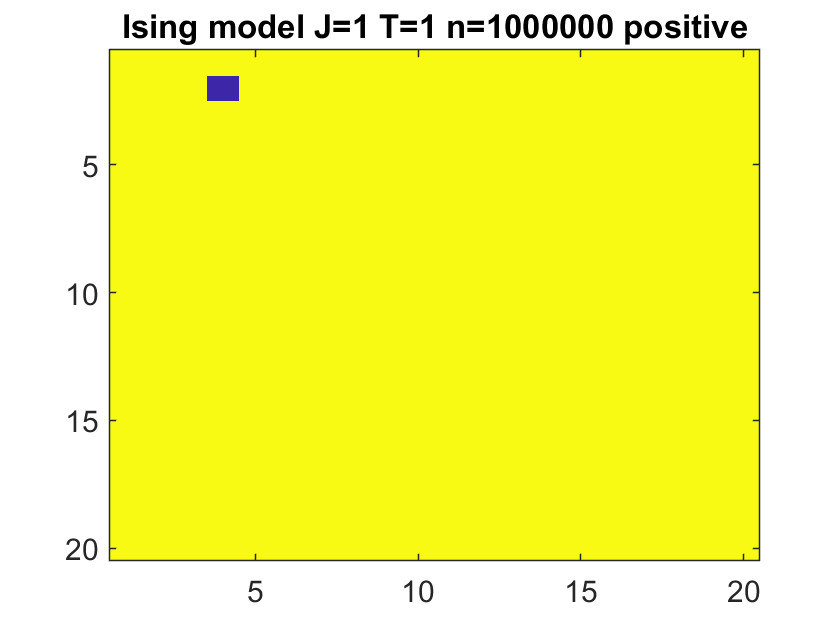
\includegraphics[width = 80mm]{st1n6p.png}
\end{minipage}
\caption{The development of spin latice of the Ising model using Markov chain Monte Carlo simulation. $J=k_B=1$, $T=1$. The program is run for $N=10^6$ steps. Here the states for step $n=0,10^2,10^4,10^6$ are taken as examples. From the plots, it can be implied that at this temperature, spins of the same sign will spontaneously concentrate and at last get nearly completely magnetized to a particular sign. For these plots, the system at last gets completely magnetized to a positive $M$. In this figure, blue correspond to $s_i=1$, and yellow is $s_i=-1$.}
\label{fig:st1p}
\end{figure}

\clearpage

The magnetization as a function of steps $M-n$ for the two results are given respectively in Fig. \ref{fig:mt1n} and Fig. \ref{fig:mt1p}.\par

\begin{figure}[ht]
\centering
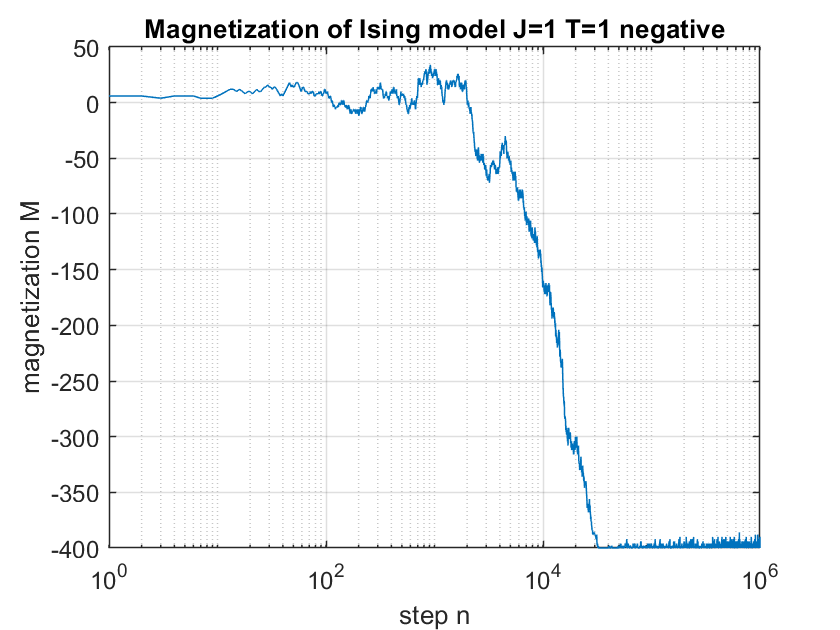
\includegraphics[width = 120mm]{mt1n.png}
\caption{The magnetization $M$ as a function of steps $n$ for the Markov chain Monte Carlo simulation of Ising model. $J=k_B=1$, $T=1$. The program is run for $N=10^6$ steps. It is apparent that the system get spontaneously magnetized at some time after enough time. It can also be implied from this plot that at $T=1$, the magnetization is complete and stable. Once the system starts to get highly magnetized, it is hard to flip the sign of $M$ then. Once $M\to\mathrm{M_{max}}$, it will keep staying there later. This plot shows the result of a negative megnetization at last.}
\label{fig:mt1n}
\end{figure}

From these two plots we can imply that, for $T=1$, spontaneous magnetization exists and is complete and stable after long enough time. When at first $M$ is small, it is possible that $M$ will flip sign by random spin flipping. But when at some time, spins of the same sign start to concentrate, and in this case, as the absolute value of $M$ gets larger, spins will tend to flip to the majoarity sign, since the probability of accaptance of the contrary move will get smaller and smaller, until almost all the spins are of the same sign, either negative or positive. At this time, it is hignly impossible that another flip will be accepted, thus making the magnetization complete and stable.\par

\begin{figure}[ht]
\centering
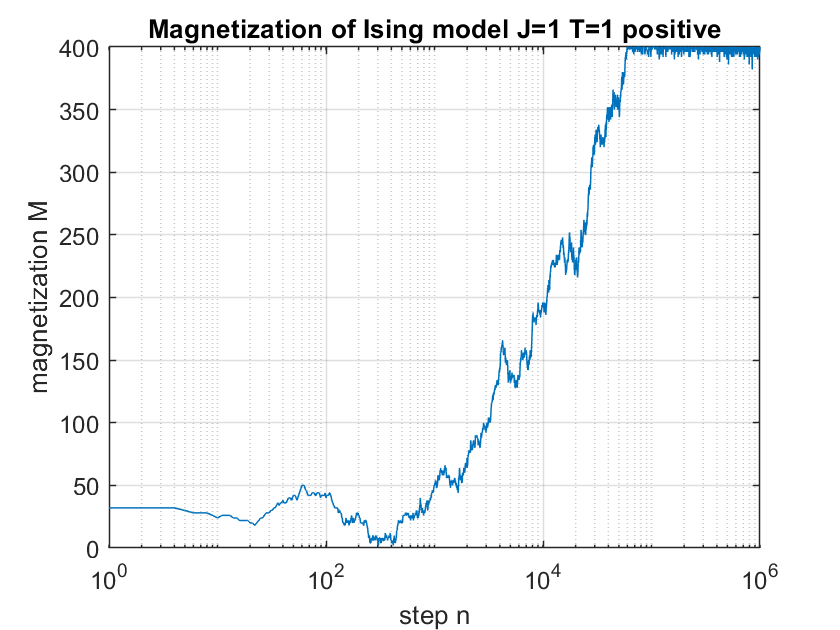
\includegraphics[width = 120mm]{mt1p.png}
\caption{The magnetization $M$ as a function of steps $n$ for the Markov chain Monte Carlo simulation of Ising model. $J=k_B=1$, $T=1$. The program is run for $N=10^6$ steps. It is apparent that the system get spontaneously magnetized at some time after enough time. It can also be implied from this plot that at $T=1$, the magnetization is complete and stable. Once the system starts to get highly magnetized, it is hard to flip the sign of $M$ then. Once $M\to\mathrm{M_{max}}$, it will keep staying there later. This plot shows the result of a positive megnetization at last.}
\label{fig:mt1p}
\end{figure}

Therefore, $T=1$ should be far below the critical temperature, while the exact sign of $M$ in the end should be random, as seen from several results got.\par
Then we will go to $T=2,3$ and see what will happen. The plots of magnetization for these two temperatures are Fig. \ref{fig:mt2} and Fig. \ref{fig:mt3} repectively.\par
When $T=2$, according to Fig. \ref{fig:mt2}, $M$ will grow to some non-zero value and stay arround the value for a long time, indicating the existance of spontaneous magnetization. However, compared to $T=1$, now $M$ oscillates a bit strongly around the value. At $n\approx10^5$, we can see several spikes, which means $M$ for many times nearly got fliped to the opposite sign. From Fig. \ref{fig:st23} we can see the distribution of opposite spins, so we can reasonably guess that at some time, by random flipping, the distribution of opposite spins are somewhat concentrated, and thus may allow a higher probability to accept more opposite flippings, which will result in the change of the sign of $M$. For $T=1$, the number of opposite spins is too small, so that it is extremely hard to flip the sign of $M$ after complete magnetization. Therefore, it may be implied that $T=2$ is lower than but close to the critical temperature of spontaneous magnetization.\par
When $T=3$, according to Fig. \ref{fig:mt3}, $M$ oscillates seriously around 0 instead of a non-zero number. In the plot we cannot see any platforms which indicate spontaneous magnetization. Therefore, we may imply that for this temperature, spontaneous magnetization does not exist. To further prove it, $M$ is averaged over the whole process, and the average is $\bar{M}=-0.7438\approx0$. Therefore, $T=3$ should be larger than the critical temperature. Similarly, $\bar{M}(T=2)=69.8115$, $\bar{M}(T=1,+)=391.8086$, $\bar{M}(T=1,-)=-393.6338$. So as temperature grows from lower than the critical temperature, the magnetization will decrease, until when larger than $T_c$, $M\to 0$. This satiesfies what we have learnt in solid state physics course about magnetization.\par

\begin{figure}[ht]
\centering
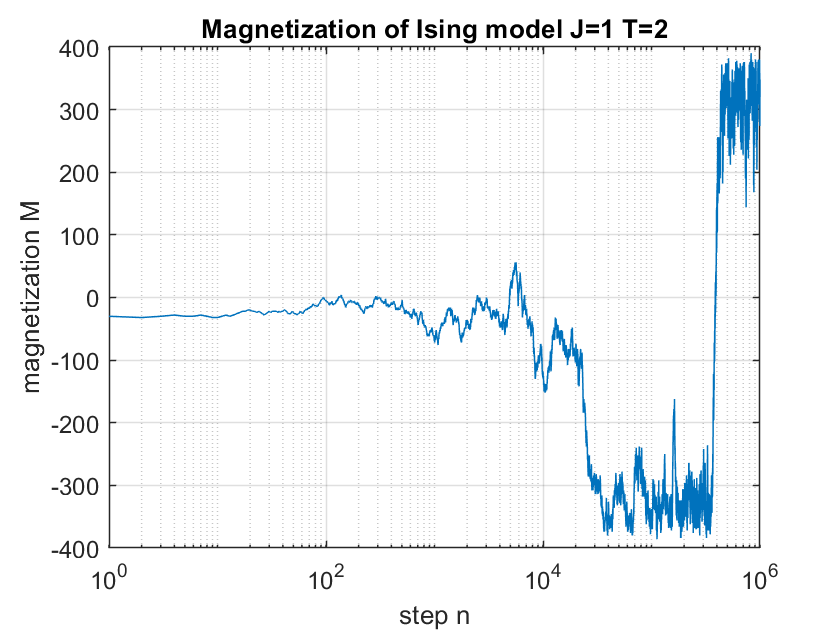
\includegraphics[width = 120mm]{mt2.png}
\caption{The magnetization $M$ as a function of steps $n$ for the Markov chain Monte Carlo simulation of Ising model. $J=k_B=1$, $T=2$. The program is run for $N=10^6$ steps. For $T=2$, spontaneous magnetization still exists, since $M$ will reach a large value and stay for not a short time. However, compared to $T=1$, for $T=2$, $M$ can get large, over three quarters of the maximum, but will oscillate much stronger and is also able to get flipped even after spontaneous magnetization. According to Fig. \ref{fig:st2}, it can be guessed that at some time after magnetization, the opposite spins may gather, providing higher probability to accept opposite spin flipping. It may be partially proved by the sevaral spikes arround $n=10^5$, but to further prove the flipping condition, spin lattice plots like above should be provided, but it is hard to get without the help of movies, since we cannot predict when $M$ will flip. From the result, we may imply that $T=2$ should be smaller than but close to the critical temperature.}
\label{fig:mt2}
\end{figure}

\begin{figure}[ht]
\centering
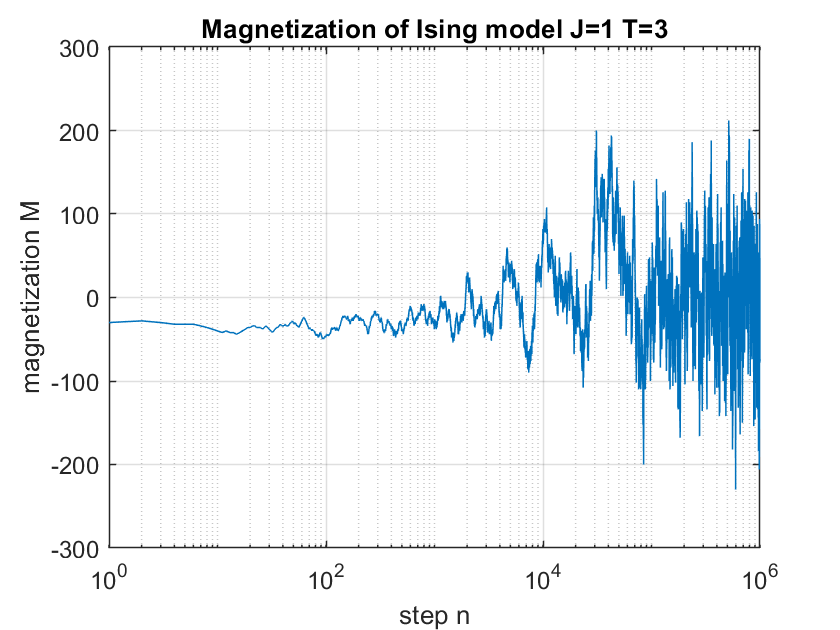
\includegraphics[width = 120mm]{mt3.png}
\caption{The magnetization $M$ as a function of steps $n$ for the Markov chain Monte Carlo simulation of Ising model. $J=k_B=1$, $T=3$. The program is run for $N=10^6$ steps. For $T=3$, spontaneous magnetization cannot be seen from the steps we have calculated since $M$ won't grow to a none-zero value and stay for quite a while. In this plot, we can see that the system is highly oscillatory after enough time and will not stay arround some certain non-zero values as a platform, at least within our time range. However, since $N=10^6$ seems already long enough, so we may conclude that $T=3$ should be higher than the critical temperature.}
\label{fig:mt3}
\end{figure}

\begin{figure}[ht]
\centering
\begin{minipage}{0.48\linewidth}
\centering
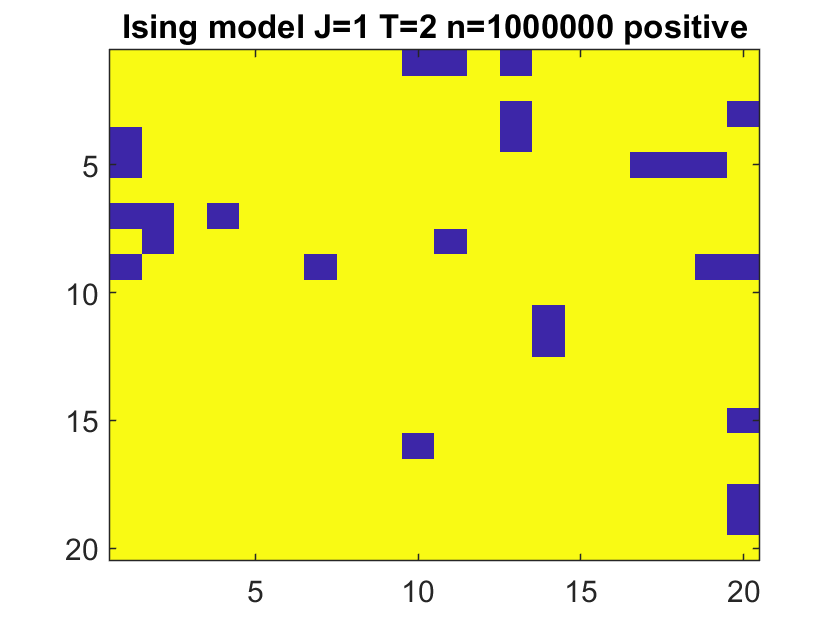
\includegraphics[width = 80mm]{st2n6.png}
\end{minipage}
\begin{minipage}{0.48\linewidth}
\centering
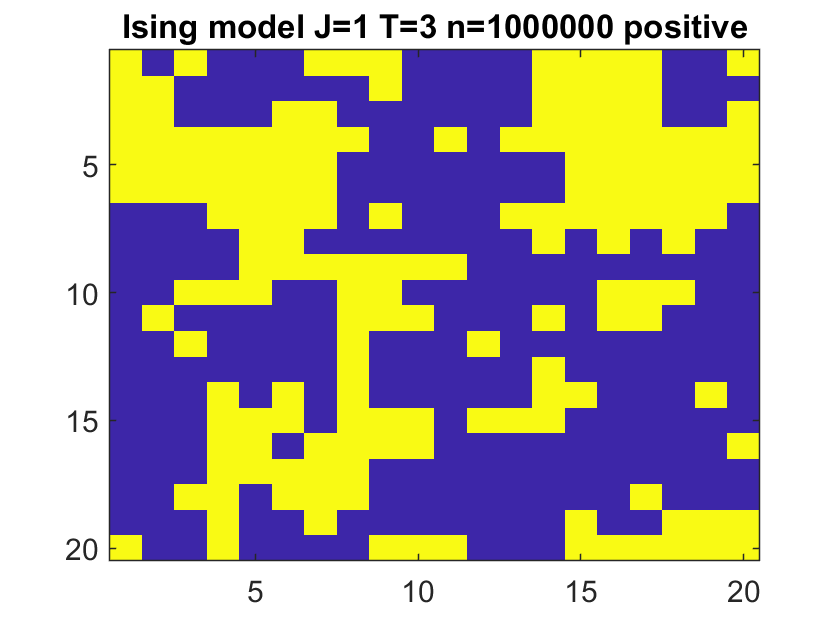
\includegraphics[width = 80mm]{st3n6.png}
\end{minipage}
\caption{The development of spin latice of the Ising model using Markov chain Monte Carlo simulation. $J=k_B=1$, $T=2, 3$. The program is run for $N=10^6$ steps. Here provides the spin distribution for the last step. For $T=2$, from the plot, it can be implied that the system is magnetized, and the opposite spins are randomly distributed. With enough amount of opposite spins, at some random time, these opposite spins may gather, providing higher probability to flip the sign of $M$. Moreover, the opposite spins decreases the average magnetization. For $T=3$, both signs of spin are always uniformly randomly distributed, indicating no spontaneous magnetization. In this figure, blue correspond to $s_i=1$, and yellow is $s_i=-1$.}
\label{fig:st23}
\end{figure}

\clearpage

\section*{Problem 2}
\subsection*{a)}
The code to simulate the dimer covering problem using simulated annealing method is available in \textquotedblleft Hw\_6-2.c\textquotedblright. Similar to Prob. 1, here we still make a move each time if accepted, but now to get the ground state, we start with a high temperature and gradually cool down to nearly 0, while in Prob. 1, the temperature is constant. \par
In dimer covering problem, for each move we choose an adjacent pair of sites from the $50\times50$ lattice. If the pair is completely not occupied, then we directly add a dimer here, since it will lower the energy, i.e. the opposite of the total number of dimers covered $E=-n_\mathrm{dimer}$. Or if the pair of sites are occupiecd by a single dimer, then we will remove it with Boltzmann probability
\begin{equation}
P_\mathrm{a}=\mathrm{e}^{-1/T}
\label{eq:pacc}
\end{equation}
Here we set Boltzmann constant $k_\mathrm{B}=1$, and $E_j-E_i=1$ for removing one dimer. And otherwise, we do nothing to the system.\par
if we start with an initial temperature $T_0$, then the cooling procedure, i.e. the temperature $T$ for each step $n$, will be
\begin{equation}
T=T_0\mathrm{e}^{-n/\tau}
\label{eq:T}
\end{equation}
where $\tau$ is a time constant which determines the speed of cooling.\par
In this problem, we choose the initial temperature $T_0=10$, and change the value of time constant $\tau$ to see the solution and how the solution depends on the cooling procedure chosen. The values of $\tau$ tested are 10, 100, 1000, 5000, 10000, and 100000.\par
To see the result of covering, dimer coverage of an early state $t=100$, and the final state for $\tau=1000$ is plotted in Fig. \ref{fig:d}. In the early state we can see clearly how dimers start covering the lattice, and in the final state of $n=100000$, nearly all the sites are covered with dimers, which agrees with the theoretical prediction that the ground state is when all the sites are covered by dimers.\par

\begin{figure}[ht]
\centering
\begin{minipage}{0.48\linewidth}
\centering
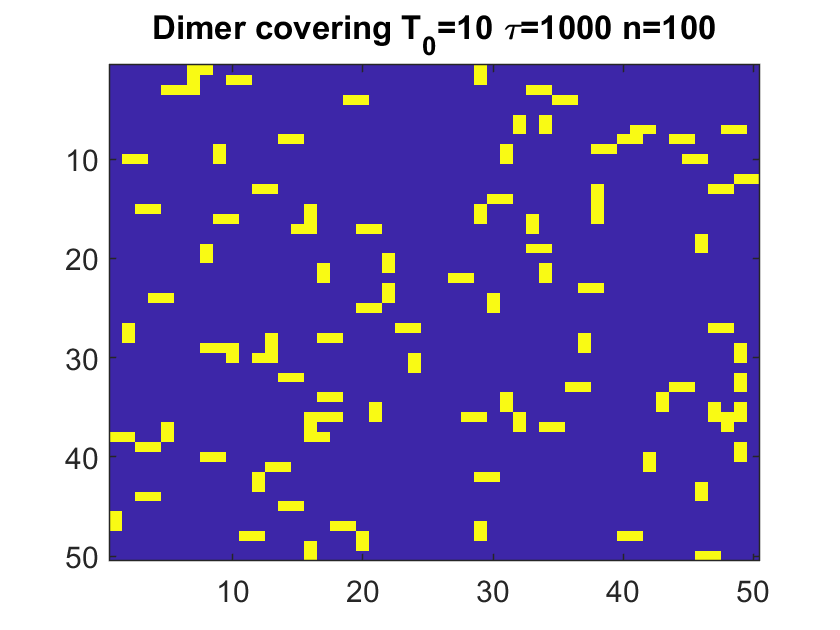
\includegraphics[width = 80mm]{ds.png}
\end{minipage}
\begin{minipage}{0.48\linewidth}
\centering
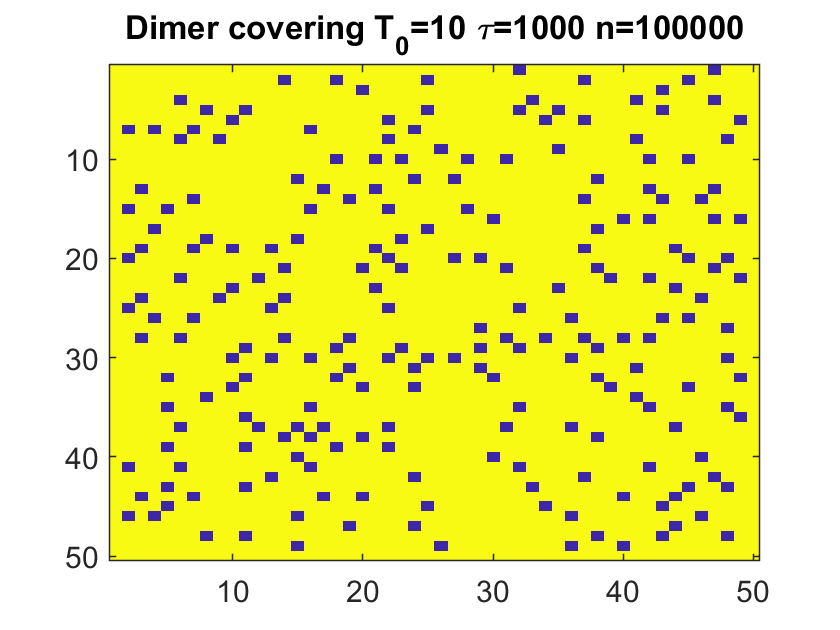
\includegraphics[width = 80mm]{df.png}
\end{minipage}
\caption{Dimer coverage of an early state $n=100$, and the final state, for $\tau=1000$. In the early state we can see clearly how dimers start covering the lattice. And in the final state of $n=100000$, nearly all the sites are covered with dimers, which agrees with the theoretical prediction that the ground state is when all the sites are covered by dimers, although not perfect.}
\label{fig:d}
\end{figure}

\subsection*{b)}
Then to see how cooling schedule affects the solution, the developments of energy with respect to steps $n$ for all the time constants $\tau$ chosen are plotted together in Fig. \ref{fig:de} with logarithmically-spaced time intervals. For $\tau=10,100$, the development of energy is nearly the same, while $\tau=10$ is a bit faster at first but is soon caught up by $\tau=100$. When the cooling schedule keeps slowing down, for $\tau=1000,5000,10000,100000$, the decrease of energy is a just bit slower at the beginning, compared with fast cooling, but soon at several thousand steps, a platform of $E\approx800$ appears for all slow schedules. And then the slower the schedule is, the later the energy starts falling again.\par

\begin{figure}[ht]
\centering
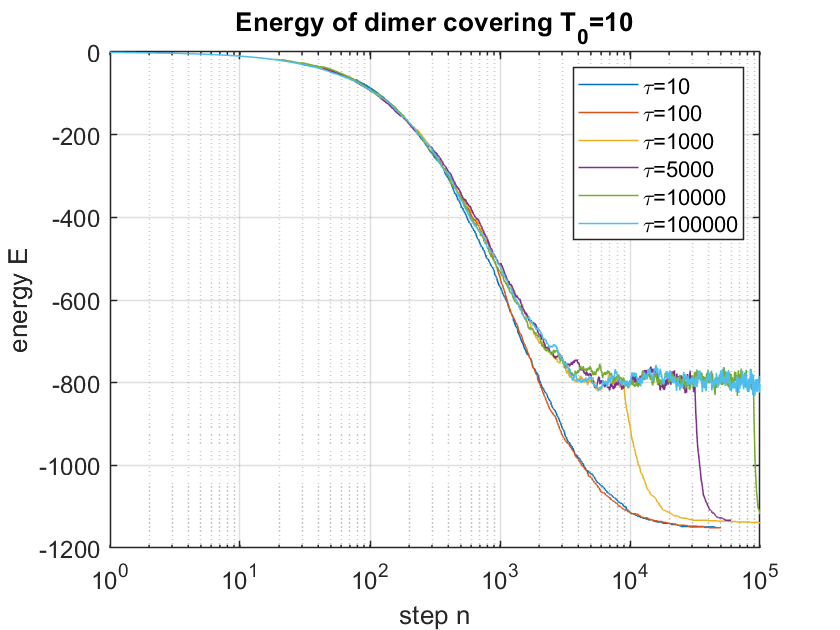
\includegraphics[width = 110mm]{de.png}
\caption{Energy with respect to steps $n$ for $\tau=10, 100, 1000, 5000, 10000$. For $\tau=10,100$, the two procedures are nearly the same. When $\tau$ gets larger, the decrease of energy is a just bit slower at the beginning, but soon at $n\approx3000$, a platform of $E\approx800$ appears for all $\tau$'s. Then the slower the schedule is, the later $E$ starts falling again.}
\label{fig:de}
\end{figure}

Although for this simple problem, it seems that fast cooling is still good since they all reaches to nearly the same result $E\approx1150$, which is quite close to the true result 1250, though not perfect, due to the hardness to remove and add dimers at very low temperature, according to Eq. \ref{eq:T}, it requires a much lower temperature for fast cooling to get the same result as the slower ones. 

\section*{Problem 3}
\subsection*{a)}
Linear congruential random number generator (LCG) to generate uniformly distributed random numbers $r$ between $[0, 0.1)$ is as follows
\begin{equation}
\begin{gathered}
x'=(ax+c)\,\mbox{mod}\: m\\
r=x/m
\end{gathered}
\label{eq:LCG}
\end{equation}
In the following simulation, we choose the constants given in Newman's book: $a=1664525$, $c=1013904223$, $m=2^{32}=4294967296$. The initial value of $x$ is chosen by the time. During the whole simulation of 10000 random Gaussian numbera, 20000 uniformly distributed random numbers are generated by this LCG. These random numbers is plotted in Fig. \ref{fig:lcg} with respect to steps. It is clear that the output seems uniformly random. 

\begin{figure}[ht]
\centering
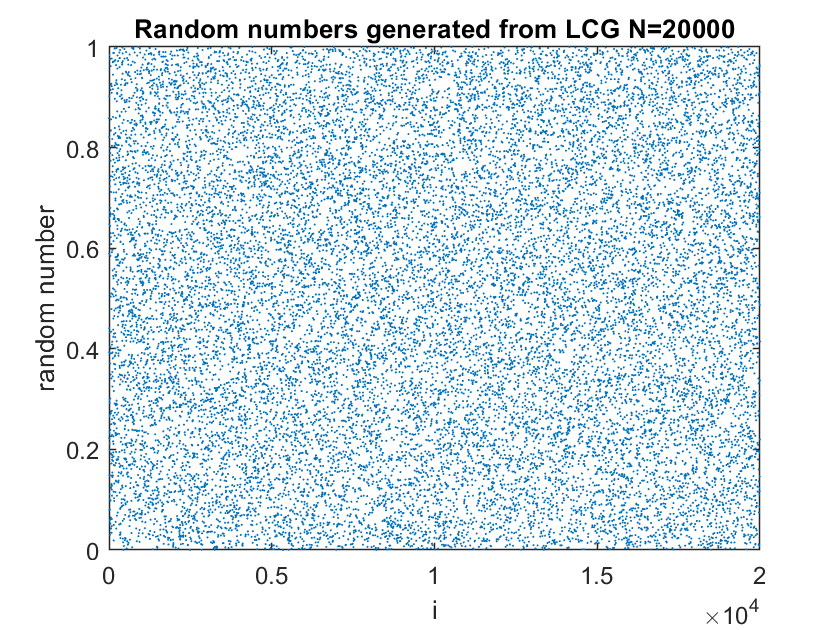
\includegraphics[width = 110mm]{lcg.png}
\caption{Linear congruential random number generator (LCG) to generate uniformly distributed random numbers $r$ between $[0, 0.1)$ by $x'=(ax+c)\,\mbox{mod}\: m$, $r=x/m$ iteratively. Here the value of constants are chosen from Newman's book: $a=1664525$, $c=1013904223$, $m=2^{32}=4294967296$. The initial value of $x$ is chosen by the time. This plot shows the first 20000 numbers generated with $x_0=1578719623$. This plot indicates the (psudo-)randomness and uniformity as said.}
\label{fig:lcg}
\end{figure}

\subsection*{b)}
As provided by the textbook, to generate random Gaussian numbers with zero mean and standard diviation $\sigma$ from uniformly distributed random numbers within $[0,1)$, we may follow Eq. \ref{eq:rg}
\begin{equation}
\begin{gathered}
r=\sqrt{-2\sigma^2\ln(1-z)}\\
\theta=2\pi z\\
x=r\cos\theta
\end{gathered}
\label{eq:rg}
\end{equation}
Here $z\in[0,1)$ is a uniformly distributed random variable.\par
This problem chooses $\sigma=1$, i.e. unit Gaussian, as an example. 10000 random Gaussian numbers are generated in the way mentioned. To show that the frequency is correctly calculated, we plot the histogram with a proper bar width 0.1, and compare the frequency with the theoretical probability distribution. For the original histogram, the amount of each bar is the total amount of random numbers within the bar's range. Then the probability to get into a range is the amount within dividen by the entire amount of numbers generated. To get the true normalized histogram, we still have to divide the values by the bar width, since for small width $\Delta x$ the relationship between the probability in an interval and the frequency there is
\begin{equation}
p([x,x+\Delta x])=f(x)\Delta x
\end{equation}
where $f(x)$ is the frequency or probability distribution function. The probability distribution function for the unit Gaussian is
\begin{equation}
f(x)=\frac{1}{\sqrt{2\pi}}\mathrm{e}^{-\frac{1}{2}x^2}
\label{eq:unig}
\end{equation}
The histogram of the 10000 random gaussian numbers is as shown in Fig. \ref{fig:rg} with the theoretical expectation by Eq. \ref{eq:unig}. we can see that the simulation result matches very well with the expected result, except for the very rare events, there are relatively bigger difference, but still great. Another histogram in the same condition of 100000 numbers is added to the figure. For larger amount of random numbers, the probability distribution matches even better. 

\begin{figure}[ht]
\centering
\begin{minipage}{0.48\linewidth}
\centering
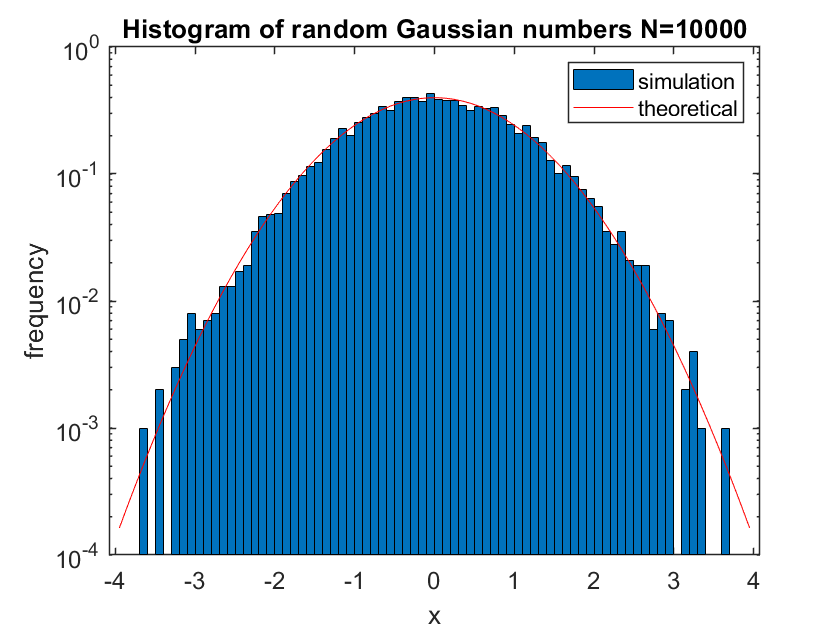
\includegraphics[width = 80mm]{rg4.png}
\end{minipage}
\begin{minipage}{0.48\linewidth}
\centering
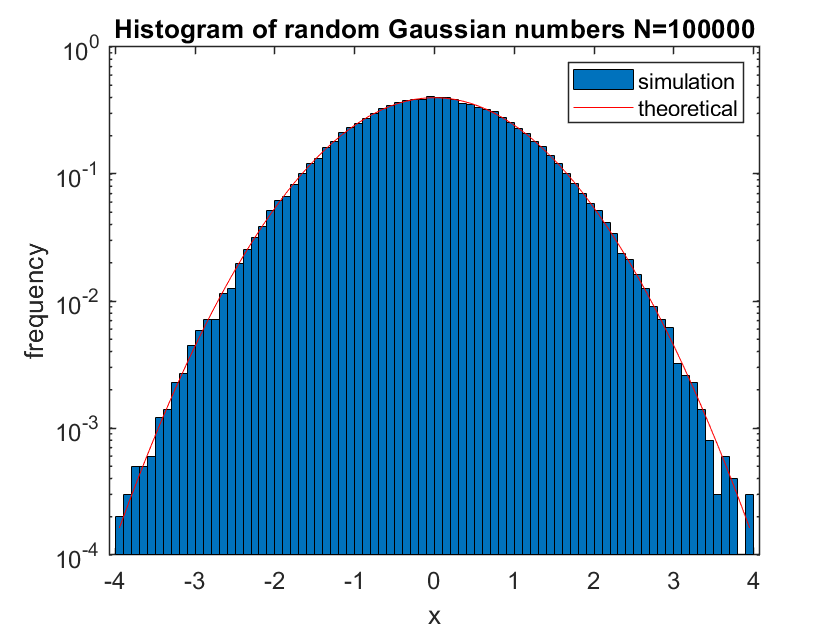
\includegraphics[width = 80mm]{rg5.png}
\end{minipage}
\caption{Normalized histogram of the unit random Gaussian numbers generated. The histograms are drawn in the range $x\in[-4,4]$, with bar width $\Delta x=0.1$. For $N=10000$, the histogram already matches with the expectation $f(x)=\frac{1}{\sqrt{2\pi}}\mathrm{e}^{-\frac{1}{2}x^2}$ very well for most $x$, except for large $|x|$. the frequency of rare events agrees much better with the theory.}
\label{fig:rg}
\end{figure}

\subsection*{c)}
Using the code of discrete Fourier transform (DFT) in Homework 3, we can produce the DFT $c_k$ of the random Gaussian numbers generated, and then calculate the power spectrum $P=|c_k|^2$ of these 10000 numbers. Fig. \ref{fig:psg} shows the power spectrum. From the plot we can imply that the random Gaussian number list scales correctly with wavenumber k, since for a random list, there does not exist a dominant frequancy. So the spectrum should be uniform but a bit random, just like in the figure the power speutrum is rather uniformly and in the range $P\in[10^{2.5},10^{4.5}]$, which can prove the randomness of our list generated.

\begin{figure}[ht]
\centering
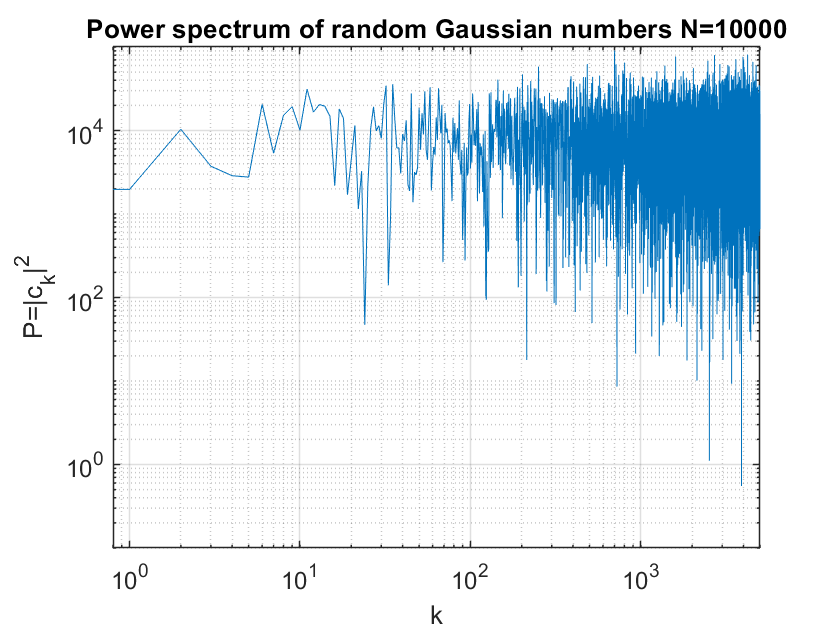
\includegraphics[width = 110mm]{psg.png}
\caption{Power spectrum of random Gaussian numbers, N=10000. Since it is obvious that the $P(k)$ lies uniformly within $[10^{2.5},10^{4.5}]$, there does not exist a dominant frequency that the $P$ is significantly larger than others. Therefore, it proves the randomness of of the list generated from Eq. \ref{eq:rg}, or say the power spectrum has the correct scaling.}
\label{fig:psg}
\end{figure}


\subsection*{d)}
From the list of random Gaussian generated above, we can construct a random walk by adding each time a random Gaussian number, or in other words, calculate the sum of (the first) $i$ random Gaussian numbers. The random walk process constructed in this way is plotted in Fig. \ref{fig:rw}.

\begin{figure}[ht]
\centering
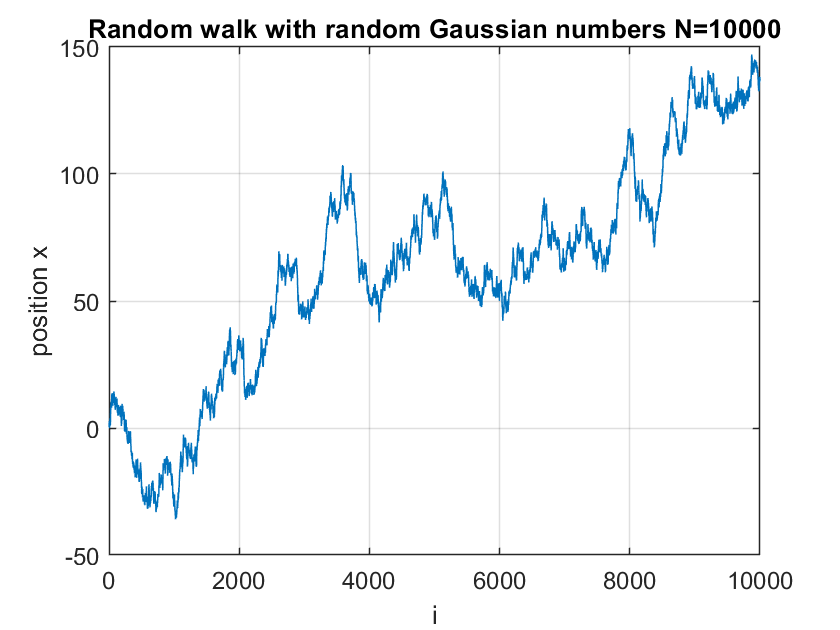
\includegraphics[width = 110mm]{rw.png}
\caption{Random walk constructed by adding a random Gaussian number each time, or in other words, summing up the first $i$ random Gaussian numbers as the position of the i'th iteration.}
\label{fig:rw}
\end{figure}

\subsection*{e)}
Similar to part c), we can also calculate the power spectrum of the random walk process. Plotted in $\log(P)$ vs. $\log(k)$ form, in Fig. \ref{fig:psrw}, it shows a clear linear relationship between $\log(P)$ and $\log(k)$, i.e. an exponential relationship between $P$ and $k$. When drawing the theoretical scaling $P\propto k^{-2}$ with the simulated power spectrum, we can see thay matches perfectly with a bit additional randomness. Therefore, the power spectrum of the simulated random walk has the correct scaling with wave number $k$.

\begin{figure}[ht]
\centering
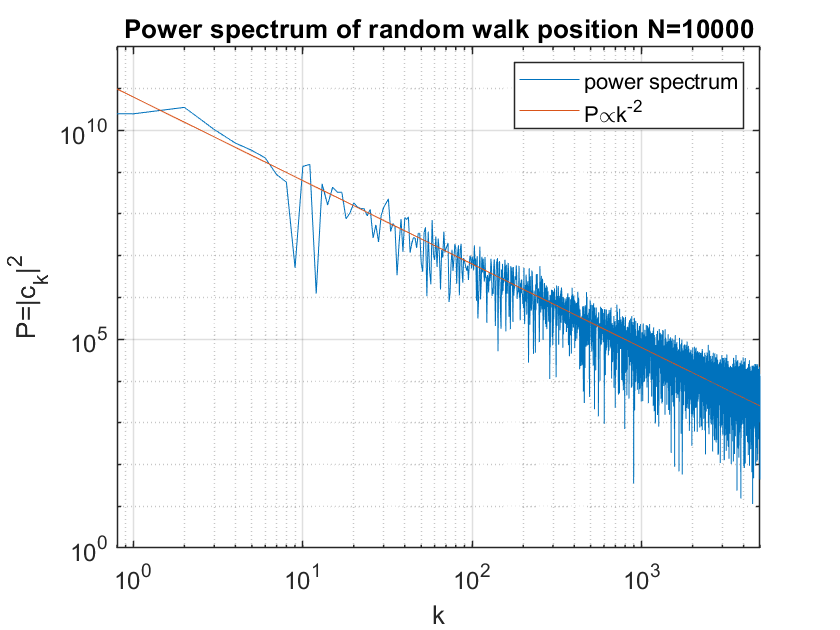
\includegraphics[width = 110mm]{psrw.png}
\caption{Power spectrum of random walks constructed using random Gaussian number list, N=10000, plotted together with the expected scalng $P\propto k^{-2}$. It is apparent that the power spectrum matches perfectly with the theoretical prediction, adding a bit of randomness to it. Therefore, it demonstrates that $P(k)$ has the correct scaling with $k$.}
\label{fig:psrw}
\end{figure}

\end{document}